\documentclass{article}

\usepackage{graphicx}
\usepackage{amsmath}
\usepackage{multirow}

\graphicspath{{plot/pdfs/}, {figs/pdfs/}}

\title{Accelerating Spike Exchange with Hardware Affinities in Parallel NEURON Simulations using Graph Partitioning}
% \author{Author}
% \date{\today}

\begin{document}

\maketitle

\begin{abstract}
In this study, we used METIS for graph partitioning on NEURON models to optimize the communication during simulation using hardware affinities.
Graphs to be used as input for METIS are generated from the communication matrix extracted from the simulation.
After the partitioning corresponding mapping from virtual processes to real hardware is calculated.
Our method is simply to map frequently communicating processes to the same machine if possible in order to decrease the overhead of communication.
Our results on a system with 80 cores shows that communication time improvements up to 17\% are possible using this method.
\end{abstract}

\section{Introduction}
\label{sec:introduction}

As the neural models grow in size simulations require larger clusters for computation.
Nowadays most neuron simulators use a parallel programming strategy for simulations.
Message Passing Interface (MPI) is commonly used for its resemblance on how neurons work.
In this schema, each neuron is represented by a separate process and spikes are exchanged between processes using communication facilities provided by MPI.

NEURON simulator use \texttt{MPI\_Allgather} and \texttt{MPI\_Allgatherv} calls for spike exchange \cite{migliore_parallel_2006}.
Using allgather calls each spike message is distributed to all other processes in the system.
Simplicity of this approach allows MPI vendors to optimize these calls in various ways.
However this strategy is not scalable as the number of processes in the system increases.

Hardware affinities are commonly used in message passing systems to increase the performance.
MPI implementations use virtual processes that are mapped to real processes either as a specified way or an arbitrary fashion.
Processes that communicate frequently are placed close to each other to decrease overhead of communication.

In this work, we tried to use METIS with NEURON to distribute virtual processes to real cores in an optimum way using hardware affinities.
First we extract the communication matrix from NEURON simulating a neural model.
Then we convert this communication matrix into an undirected weighted graph and partition this graph using METIS.
Finally we use the output from METIS to calculate the optimum placement of MPI processes on real hardware.

For the experiments, we tried to simulate a model with a number of processes equal to the number of cores on a cluster with 80 cores.
Results show improvements up to 17\% in the total communication time of the model.
We also experimented with less number of cores and less number of processes per core to see the effect of scalability.
Results comfirm that improvements are still possible although to a lesser degree.

The rest of this paper is organized as follows.
Section~\ref{sec:background} gives a background on the applications we used namely NEURON and METIS.
Our workflow is discussed in Section~\ref{sec:methodology}.
Section~\ref{sec:experiments} presents our experimental results.
Related work is given in Section~\ref{sec:related-work}.
Finally our conclusions and future work can be found in Section~\ref{sec:conclusions}.

\section{Background}
\label{sec:background}

In this section we give a brief background on the applications we use for this study.

\subsection{NEURON}

NEURON is a simulation environment for modeling individual neurons or networks of neurons \cite{hines_neuron_1997}.
It provides convenient tools to construct, exercise and manage models without requiring experience in numerical methods or programming.
It has been an important tool for computational neuroscience and has been used in numerous scientific studies.

Although initially developed for single-cell models running on a single machine, it has been extended to support multiple-cell network models distributed across different machines running in parallel \cite{migliore_parallel_2006}.
Network parallelization is implemented using Message Passing Interface (MPI).
Each processor integrates equations for a subset of the network and communicate with each other for spike exchange during simulation.

For spike exchange MPI collective communication primitives \texttt{MPI\_Allgather} and \texttt{MPI\_Allgatherv} are used.
Using these primitives each process sends its spike messages to every other processes on the network.
This provides a simple model for spike communication and has been shown to exhibit superlinear speedup using the increase in the fraction of the problem fitting into high speed cache.
However, it has also been shown that for larger networks spike communication overhead starts to dominate the benefit of high speed cache.
Therefore fine grained communication optimizations are needed to scale the models that can be simulated even further.

\subsection{METIS}

METIS is a tool for partition graphs, partitioning finite element meshes, and producing fill reducing orderings for sparse matrices \cite{karypis_fast_1998}.
It is based on various multilevel algorithms such as multilevel recursive-bisection, multilevel k-way, and multi-constraint partitioning.
It works on both weighted and unweighted graphs.
It also has a parallel implementation for large graphs.

\section{Methodology}
\label{sec:methodology}

Our workflow can be found in Fig~\ref{fig:workflow}.
We first start by running the model on NEURON without doing anything in order extract the communication matrix for the model.
For this purpose we added tracing codes to the function \texttt{nrnmpi\_spike\_exchange} to measure the number of messages exchanged between each process.
This is accomplished by summing the number of counts in \texttt{MPI\_Allgatherv} calls.
Communication layers for spike exchange in NEURON is shown in Fig~\ref{fig:callgraph}.

\begin{figure}
  \centering
  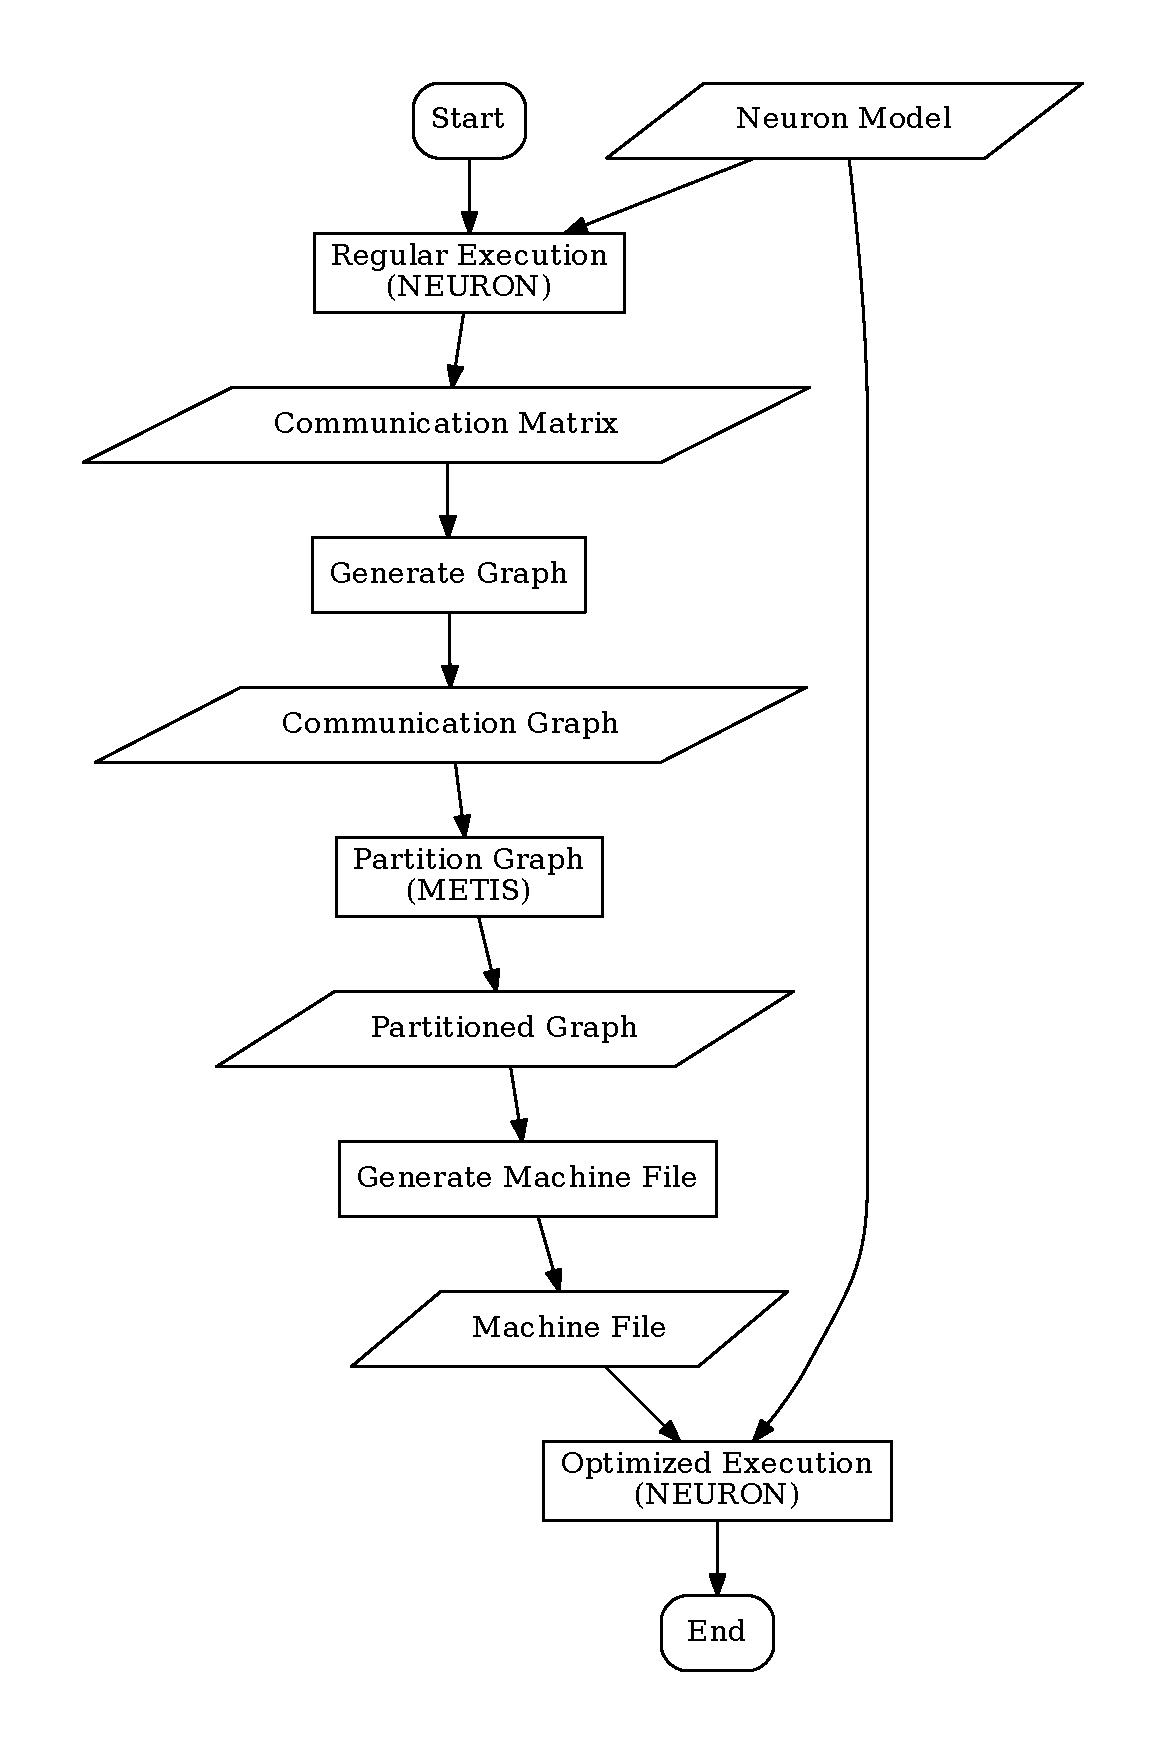
\includegraphics[width=\textwidth]{workflow.pdf}
  \caption{Our workflow}
  \label{fig:workflow}
\end{figure}

\begin{figure}
  \centering
  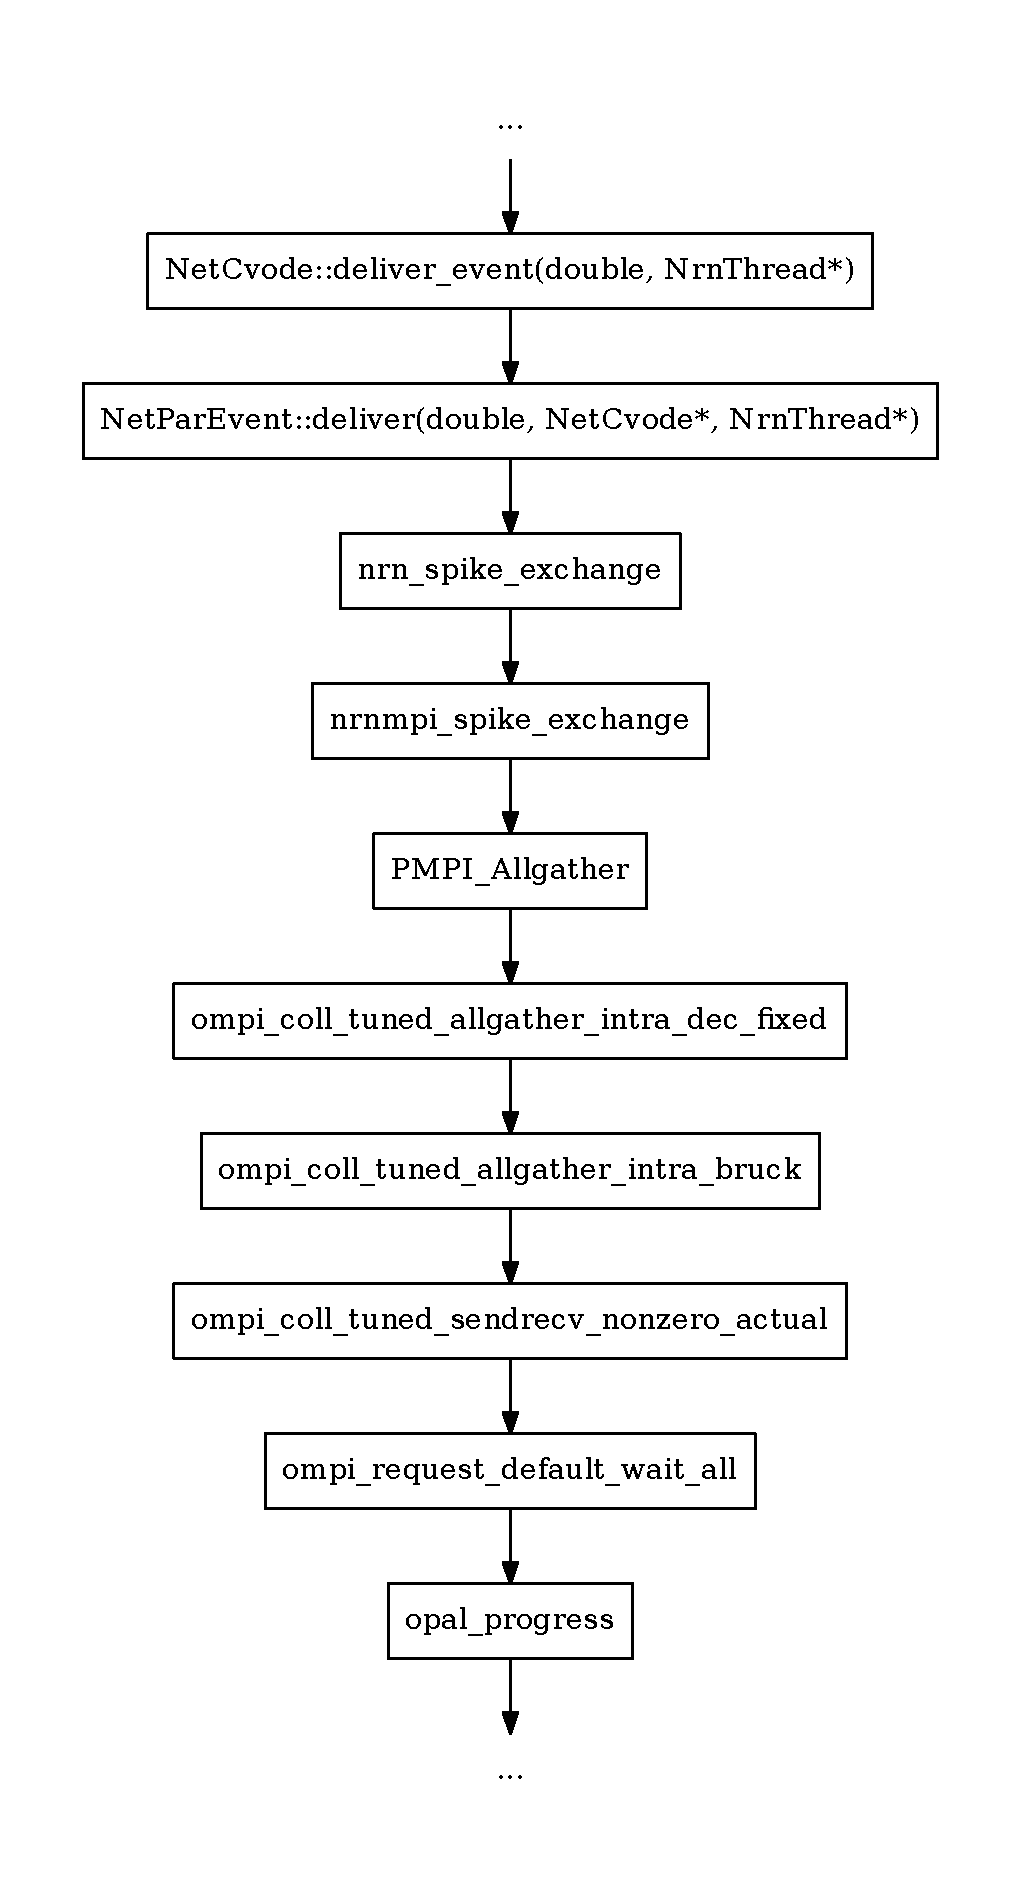
\includegraphics[width=\textwidth]{callgraph.pdf}
  \caption{Callgraph demonstrating the communication layers for spike exchange in NEURON}
  \label{fig:callgraph}
\end{figure}

After that we process this information to form a communication matrix.
In order to do that, first we use the sums we found in the previous step, $S_1, S_2, \ldots, S_n$ to form a matrix where all elements are the same in a row except for the diagonal as such:

\begin{equation*}
C = \bordermatrix{~      & P_1    & P_2    & \cdots & P_n    \cr
                  P_1    & 0      & S_1    & \cdots & S_1    \cr
                  P_2    & S_2    & 0      & \cdots & S_2    \cr
                  \cdots & \cdots & \cdots & \ddots & \cdots \cr
                  P_n    & S_n    & S_n    & \cdots & 0      \cr
}
\end{equation*}

We then sum this matrix with its transpose to add the messages received from other processes.
After that we end up with a symmetric matrix satisfying $S_{ij} = S_{ji}$ as follows:

\begin{equation*}
C = \bordermatrix{~      & P_1    & P_2    & \cdots & P_n    \cr
                  P_1    & 0      & S_{12} & \cdots & S_{1n} \cr
                  P_2    & S_{21} & 0      & \cdots & S_{2n} \cr
                  \cdots & \cdots & \cdots & \ddots & \cdots \cr
                  P_n    & S_{n1} & S_{n2} & \cdots & 0      \cr
}
\end{equation*}

From this matrix it is easy to construct a weighted undirected communication graph in the form of an input to METIS.
We then partition the graph using METIS with appropriate parameters such that each subgraph contains at most the number of cores in a single machine on the cluster we perform the experiments.
From these subgraphs we generate an MPI machine file using hardware affinities.
With this method, frequently communicating processes are preferably placed on the same machine so that communication between them will not touch the underlying network.
In the last step, we just execute the same neuron model using this machine file to compare the execution times of original and optimized versions.

\section{Experiments}
\label{sec:experiments}

In this section we present experiments with a previously published model \cite{davison_dendrodendritic_2003} obtained from ModelDB \cite{hines_modeldb:_2004}.
Parameters are changed to increase the model size to have a cell dimension array of 16 by 10 totaling up to 160 mitral cells.

\subsection{Speedups on Shared Memory}

We have used a system with 2 Intel X5660 CPU's each having 6 cores totaling up to 12 cores in order to measure the execution times on a shared memory system.
Fig.~\ref{fig:times-shared} shows the speedup plot when different number of processes are used.

\begin{figure}
  \centering
  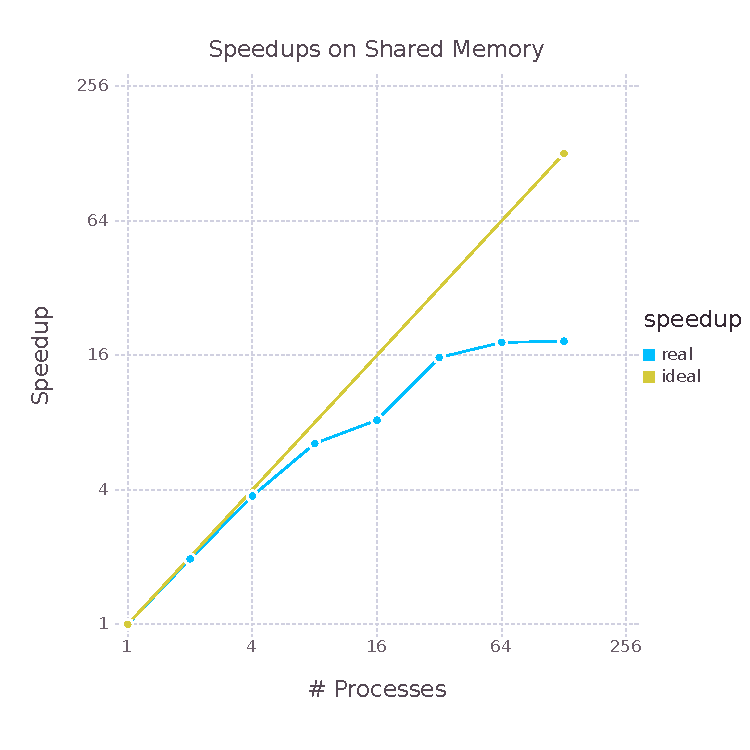
\includegraphics[width=0.7\textwidth]{times-shared.pdf}
  \caption{Speedups on a shared memory system having 12 cores}
  \label{fig:times-shared}
\end{figure}

As can be seen deviation from the ideal speedup starts as early as 4 processes.
Also note that we do not observe superlinear speedups in this system unlike the distributed memory experiments given below.
This is most likely due to the fact that every core has its own dedicated L1 and L2 caches but the L3 cache is shared between all 6 cores in this CPU model.
Since NEURON simulations are highly cache dependant this shared L3 caches limits the speedups beyond 2 processes that is 1 process for each CPU.
Nevertheless speedup rate flattens at about 16 which is more than the number of cores on the system.
This is most likely due to the use of Hyper-Threading.

\subsection{Speedups on Distributed Memory}

For distributed memory experiments we have used a cluster with 10 nodes using 2 Intel E5345 CPU's having 4 cores corresponding to 80 cores in total.
Fig.~\ref{fig:times-distributed} shows the speedup plot of the same model ran with different number of processes.

\begin{figure}
  \centering
  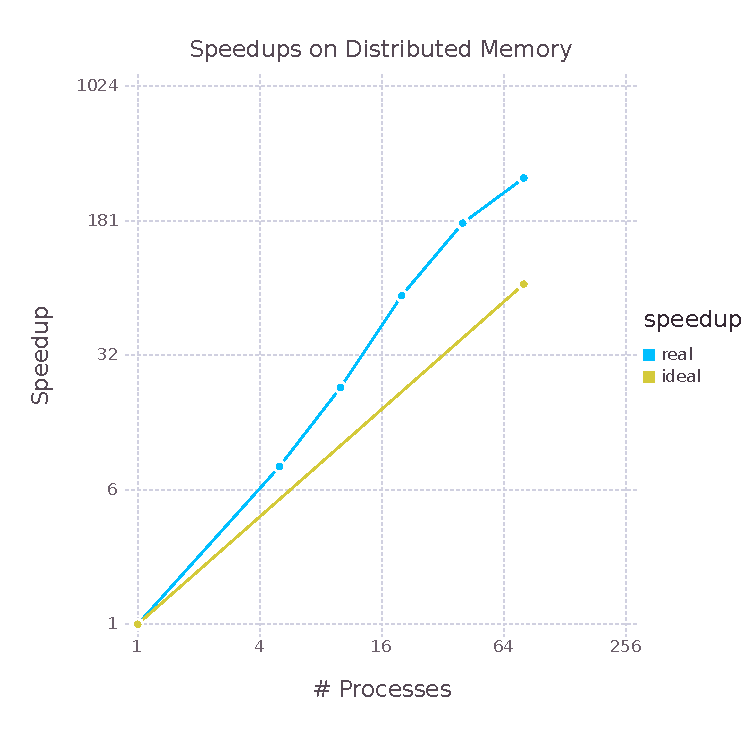
\includegraphics[width=0.7\textwidth]{times-distributed.pdf}
  \caption{Speedups on a distributed memory system with 10 nodes with 2 CPUs each having 4 cores}
  \label{fig:times-distributed}
\end{figure}

Distributed memory simulations show high amounts of super linear speedups due to the increase in the total size of cache used.
This is consistent with previous work in the literature \cite{migliore_parallel_2006}.
It is also reported that communication starts to dominate computation when the model sizes are increased.
Unfortunately we do not have access to machines to simulate these larger models.
Hence for the model sizes we used in our experiments time spent in communication is mostly negligible compared to computation.

\subsection{Integer Communication}

Integer communication is the first part of the communication during spike exchange.
Each process sends an integer number representing the number of spikes that will be sent in the second part of the communication.
This is implemented using \texttt{MPI\_Allgather} call and at each call only a single integer per process is sent.
Fig.~\ref{fig:ints} shows the total number of integers sent from a single process and all processes in total.

\begin{figure}
  \centering
  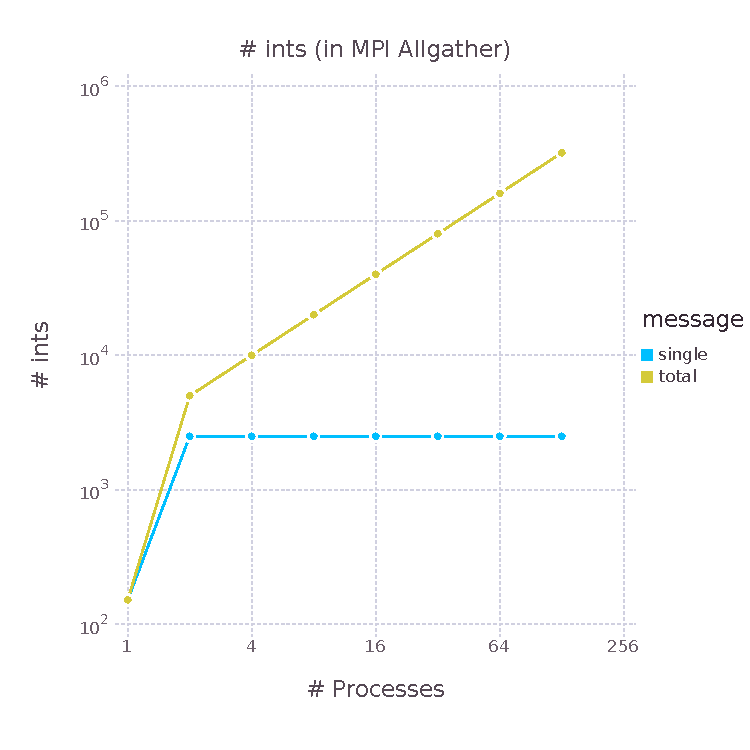
\includegraphics[width=0.7\textwidth]{ints.pdf}
  \caption{Integer communication of a single process and all processes}
  \label{fig:ints}
\end{figure}

\subsection{Spike Communication}

Spike communication is the second part of the communication during spike exchange.
In this part, actual spikes are sent to other processes using \texttt{MPI\_Allgatherv} call.
If in the first part no process decides to send a message this part is skipped.
Fig.~\ref{fig:labels} shows the total number of spikes sent from a single process and all processes in total.

\begin{figure}
  \centering
  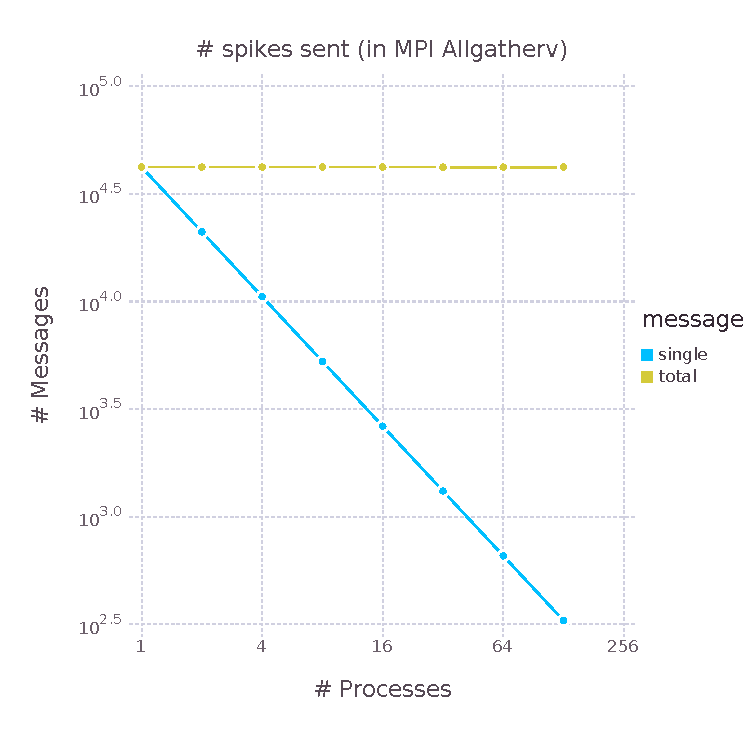
\includegraphics[width=0.7\textwidth]{spikes.pdf}
  \caption{Spike communication of a single process and all processes}
  \label{fig:labels}
\end{figure}

\subsection{Communication Matrix}

In order to see whether processes have different communication volumes we first tried to obtain a communication matrix.
Fig.~\ref{fig:comm} shows an example communication matrix obtained from a model using 80 processes.
As can be seen, some processes communicate frequently whereas others communicate less frequently.

\begin{figure}
  \centering
  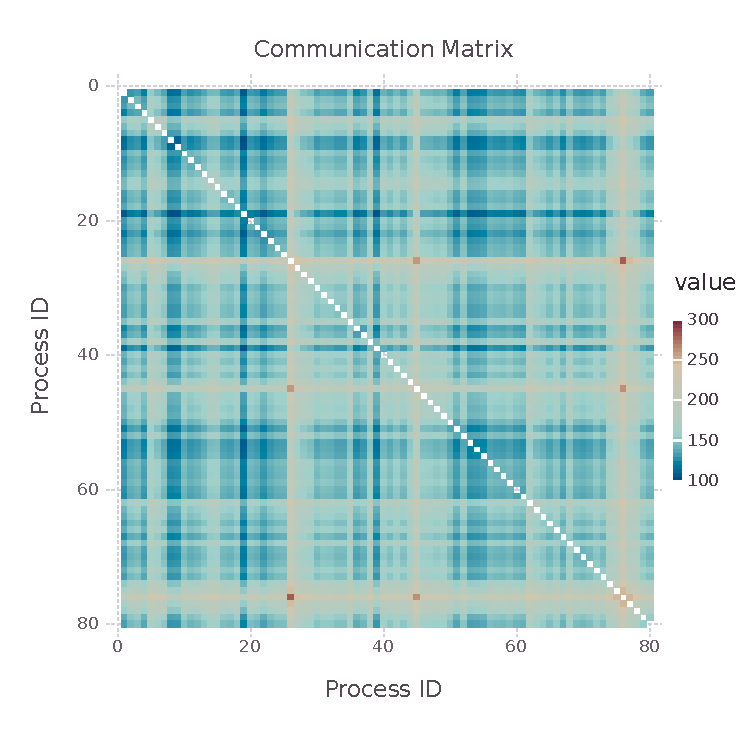
\includegraphics[width=0.7\textwidth]{communication-matrix.pdf}
  \caption{An example communication matrix with 80 processes}
  \label{fig:comm}
\end{figure}

\subsection{Execution and Communication Times}

In order to qualify the improvement of our method we measured communication times of our method and the original runs.
Experiments were done on a cluster with 10 machines each having Intel Xeon E5345 processor with 8 cores.
Fig.~\ref{fig:time} shows communication times of the original and optimized methods with different number of processes.
Tab.~\ref{tab:time} holds more detailed information including the total execution times and percentage gains with different configurations.

\begin{figure}
  \centering
  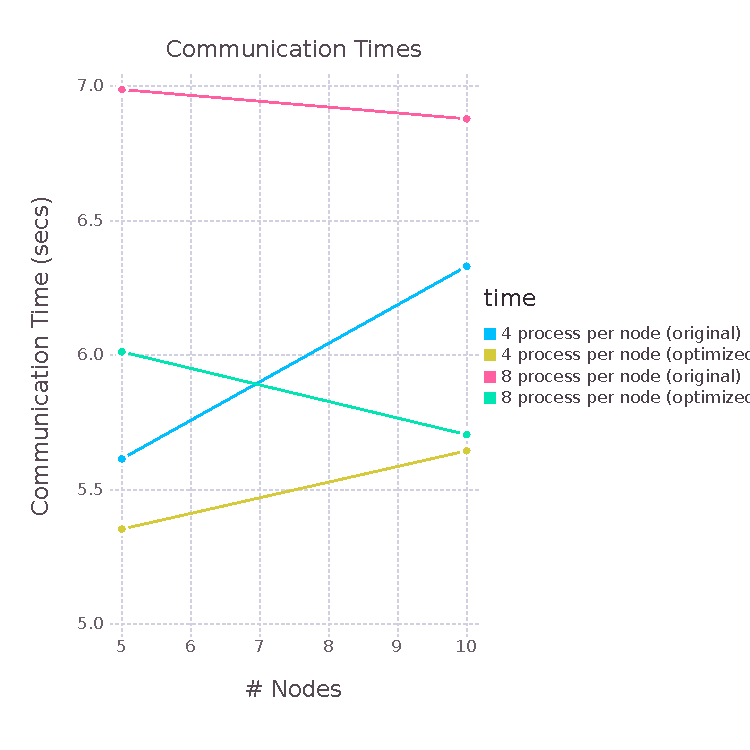
\includegraphics[width=0.7\textwidth]{communication-times.pdf}
  \caption{Communication times of the original and optimized methods with different number of processes}
  \label{fig:time}
\end{figure}

We performed experiments with 5 and 10 nodes.
In each case we compared original and optimized methods using 4 processes per node and 8 processes per node.
For each case we executed each method 5 times and take the average as the result.
When using 4 processes per node communication time seems to increase going from 5 nodes to 10 nodes.
Our method decreases the communication time by 4.6\% and 10.8\% respectively.
For 8 processes per node communication time seems to decrease going from 5 nodes to 10 nodes.
Our improvements for this case are 13.9\% and 17.0\% respectively.

\begin{table}
  \caption{Execution and Communication times with different configurations}
  \label{tab:time}
  \centering
  \begin{tabular}{|c|c|c|c|c|c|c|}
  \hline
  \# Nodes            & \# Processes per Node & Method    & Comm Time (secs) & Exec Time (secs) & Comm Impr (\%)         & Exec Impr (\%)         \\ \hline
  \multirow{4}{*}{5}  & \multirow{2}{*}{4}    & Original  & 5.615            & 171.889          & \multirow{2}{*}{4.63}  & \multirow{2}{*}{0.01}  \\ \cline{3-5}
                      &                       & Optimized & 5.353            & 171.857          &                        &                        \\ \cline{2-7} 
                      & \multirow{2}{*}{8}    & Original  & 6.988            & 102.441          & \multirow{2}{*}{13.95} & \multirow{2}{*}{1.92}  \\ \cline{3-5}
                      &                       & Optimized & 6.013            & 100.471          &                        &                        \\ \hline
  \multirow{4}{*}{10} & \multirow{2}{*}{4}    & Original  & 6.331            & 72.014           & \multirow{2}{*}{10.84} & \multirow{2}{*}{-2.10} \\ \cline{3-5}
                      &                       & Optimized & 5.645            & 73.529           &                        &                        \\ \cline{2-7} 
                      & \multirow{2}{*}{8}    & Original  & 6.879            & 38.802           & \multirow{2}{*}{17.06} & \multirow{2}{*}{-3.85} \\ \cline{3-5}
                      &                       & Optimized & 5.705            & 40.299           &                        &                        \\ \hline
  \end{tabular}
\end{table}

Note that for some configurations our method seems to increase the total execution time.
We argue that this is due to combinations of two main reasons.
First, communication times are a small portion of total execution times for the model sizes we used in our experiments.
Therefore it is difficult for our communication optimization to manifest itself in total execution times.
Second, variations in execution times for NEURON simulations are relatively high.
Sometimes one of the 5 runs takes such an extra amount of time that even if in the rest of the runs our method performs better than the original it is still worse than the original in the average.
In fact this is the case for the results using 10 nodes each running 8 processes.
Our method performs better than the original in 4 of the 5 runs but still can not make up for the last run having about a 25\% increase in the total execution time.
Nevertheless we believe that our method will begin to improve the total execution time as well when the models grow larger on bigger clusters.

\section{Related Work}
\label{sec:related-work}

Brette et al.~\cite{brette_simulation_2007} has a review study on neuron simulators.
Information about NEURON, GENESIS, NEST, NeoCortical Simulator, Circuit Simulator, XPPAUT, SPLIT, and Mvaspike can be found in the paper.
These simulators are compared according to various aspects related to simulation strategy and precision.

Migliore et al.~\cite{migliore_parallel_2006} extends NEURON simulation environment to support parallel network simulations.
MPI collective communication primitives \texttt{MPI\_Allgather} and \texttt{MPI\_Allgatherv} are used for spike exchange between processes.
It has been shown that superlinear speeedups are possible since the problem can benefit from the increase of high speed cache.
For larger networks spike exchange communication starts to dominate and becomes the limiting factor for scalability.

There are studies trying to optimize the spike exchange method employed by NEURON simulator.
Hines et al.~\cite{hines_comparison_2011} compares implementations using non-blocking multisends with naive \texttt{MPI\_Allgather} implementation on Blue Gene/P supercomputer.
This is a different approach than ours and can be combined with our method to improve the performance even further.

Broquedis et al.~\cite{broquedis_hwloc:_2010} introduced a framework named hwloc to extract hardware information from a system in a portable hierarchical manner.
This information include processors, caches, memory nodes and so on and it is used by runtime systems to adapt their communication strategies.
Paper includes experiments with both shared memory systems running on OpenMP and distributed memory systems using MPI.
MPI usage is done with two strategies.
First, information gathered through hwloc can be directly given to the process scheduler in an MPI implementation to be used for optimization.
Second, communication pattern of an application can be determined at runtime and the corresponding weighted graph representation can be generated.
This generated graph can then be combined with a second graph generated by hwloc representing the shared hierarchical memory percentage between the processors.
These graphs are then used to find the optimum static assignment of processors with a dual recursive bi-partitioning approach using SCOTCH library.

% TODO: rest of the papers

\section{Conclusions}
\label{sec:conclusions}

In this paper we proposed a method to improve communication performance in neural network simulations.
Our approach is simple and does not require modifying the source code of the simulator except for introducing tracing codes.
We also note that this method could be abstracted to be used for other distributed applications to decrease the communication overhead for better scalability.

Currently our implementation requires running the original version once in order to extract the communication matrix.
We understand that this could be a limiting factor for some applications however there are also exceptions.
Some applications have to be run multiple times such as rule checking in chip verification.
Other than that there are applications which runs in the same way but each time with different inputs.
A commonly known example for this case is the matrix multiplication performed during weather forecasting simulations.
Alternatively we believe it is also possible to break the original simulation after some time and continue in the optimized manner afterwards.
For our study we have not considered such a mechanism in order not to complicate the implementation.

We have obtained superlinear speedups in our experiments on 80 cores.
Even though the communication is a small portion of total execution on 80 cores, we expect communication to be the bottleneck with increasing number of cores.
Our future work will focus on following topics:

\begin{itemize}
  \item Performance evaluation on PRACE clusters with thousands of cores,
  \item Optimizing communication according to topological structure of the underlying network,
  \item Experiments with various examples.
\end{itemize}

\bibliographystyle{ieeetr}
\bibliography{report}
\nocite{*} % TODO: remove this

\end{document}
